\chapter{Testing del sistema}
L'attività di testing rappresenta una fase cruciale nel ciclo 
di sviluppo del software, in quanto garantisce la qualità, 
l'affidabilità e la robustezza del sistema. Questo capitolo 
illustra l'approccio metodologico e gli strumenti utilizzati per 
la verifica del corretto funzionamento del sistema.

Il testing é stato organizzato su due livelli: test unitari per
testare in isolamento la business logic; test di API tramite collection
di Postman. Tuttavia, il test di API é ancora in fase di sviluppo ed
é pertanto incompleto. Le collection sono, ad oggi, uno strumento per
gli sviluppatori per provare il funzionamento degli endpoint in modo rapido.
É previsto di rendere le collection degli effettivi test di API.

\section{Testing unitario}
Il concetto di unitá é da sempre flessibile: le unitá vanno definite
in base al contesto. Nel contesto di un sistema come DietiEstates25, é
una scelta comune quella di considerare i Service e le funzioni ausiliare
le unitá di testing.
Il testing dei Service permette di testare il funzionamento della business
logic. É anche importante specificare che, nel testing di un software sviluppato
su un framework come Spring Boot, testare meccanismi forniti da Spring Boot o
moduli terzi é chiaramente inutile.
Il testing delle funzioni ausiliare permette di assicurarsi che tali funzioni,
spesso largamente utilizzate nel codice, siano corrette. La correttezza di tali funzioni
permette di risparmiare potenzialmente tanto tempo in fase di debugging.

Si è deciso di usare una libreria di faking (Faker) per aumentare la casualitá dei campioni.

A valle di queste considerazioni, descriviamo il testing effettuato.
I test sono stati creati attraverso la piattaforma JUnit5.
\subsection{JwtUtil.isTokenValid}
Questo metodo della classe di gestione di JWT é di cruciale importanza per quanto
riguarda l'intero sistema di autorizzazione del backend.

\begin{table}[h!]
    \centering
    \renewcommand{\arraystretch}{1.4}
    \begin{tabularx}{\textwidth}{|X|X|X|}
    \hline
    \textbf{Parametro} & \textbf{Classe di Equivalenza} & \textbf{Validità} \\
    \hline
    \texttt{token} & Stringa vuota & Non valida \\
    \hline
    \texttt{token} & Token valido & Valida \\
    \hline
    \texttt{token} & Token non valido & Non valida \\
    \hline
    \texttt{token} & Token scaduto & Non valida \\
    \hline
    \texttt{UserDetails} & UserDetails valido & Valida \\
    \hline
    \end{tabularx}
    \caption{Classi di equivalenza per il testing black-box dei parametri \texttt{token} e \texttt{UserDetails}}
\end{table}

Note: 
\begin{list}{$\cdot$}{}
    \item Poiché isTokenValid viene chiamata una volta che si è 
    verificato che token è diverso da null in JwtAuthFilter, si 
    è deciso di evitare il testing sulla classe di equivalenza 
    null.
    \item Poiché isTokenValid viene chiamata una volta che si è 
    verificato che UserDetails è diverso da null (dal metodo 
    loadUserByUsername(username) di UserDetails invocato in 
    JwtAuthFilter), si è deciso di evitare il testing sulla 
    classe di equivalenza null.
    \item Si è deciso di creare una classe copia per il testing 
    a causa della non iniettabilità, per motivi di sicurezza, 
    della classe di produzione.
\end{list}

\noindent
I casi di test, secondo strategia R-WECT, sono:
\begin{table}[h!]
    \centering
    \renewcommand{\arraystretch}{1.4}
    \begin{tabularx}{\textwidth}{|X|X|X|}
    \hline
    \textbf{Token} & \textbf{UserDetails} & \textbf{Risultato Atteso} \\
    \hline
    Stringa vuota & UserDetails valido & \texttt{InvalidTokenException} \\
    \hline
    Token valido & UserDetails valido & \texttt{true} \\
    \hline
    Token scaduto & UserDetails valido & \texttt{InvalidTokenException} \\
    \hline
    Token non valido & UserDetails valido & \texttt{InvalidTokenException} \\
    \hline
    \end{tabularx}
    \caption{Casi di test secondo la strategia R-WECT}
\end{table}

\newpage
\lstinputlisting[
    style=javaStyle, 
    caption={La classe di testing per JwtUtil.isTokenValid}, 
]{assets/code/jwt-test.java}
    
\subsection{AgentReviewService::createAgentReview}
AgentReviewService::createAgentReview(AgentReviewDto, UserDetails) é invocato in contesti in 
cui UserDetails é sempre ben definito, ovvero sempre diverso da null e sempre contenente 
informazioni di utente esistente.
AgentReview Dto è costituito da:
\begin{list}{$\cdot$}{}
    \item agentId: é garantito dal validator (Hibernate Validator) che non sia null o empty-string
    \item value: é garantito dal validator che non sia null e che sia compreso tra 1 e 5
    \item comment
\end{list}

È stato scelto, per la definizione dei casi di test, un approccio functionality-based, 
in modo da considerare solo i casi di test reali. I casi di test sono:
\begin{table}[h!]
    \centering
    \renewcommand{\arraystretch}{1.4}
    \begin{tabularx}{\textwidth}{|X|X|}
    \hline
    \textbf{Agent ID} & \textbf{Risultato Atteso} \\
    \hline
    Agent ID errato & \texttt{EntityNotExistsException} \\
    \hline
    Agent ID corretto & \texttt{AgentReview} \\
    \hline
    \end{tabularx}
    \caption{Casi di test per Agent ID}
\end{table}

\newpage
\lstinputlisting[
    style=javaStyle, 
    caption={La classe di testing per AgentReviewService::createAgentReview}, 
]{assets/code/agent-review-test.java}
    
\subsection{StarredListingService::addStarredListing}
StarredListingService::addStarredListing(String userEmail, String listingId) é invocato 
in contesti in cui la validitá di userEmail é garantita. Per quanto riguarda 
listingId, il validator garantisce che, al momento della chiamata di 
questo metodo, listingId sia non nulla e non vuota.

A questo punto, le classi di equivalenza da considerare per listingId sono:
\begin{table}[h!]
    \centering
    \renewcommand{\arraystretch}{1.4}
    \begin{tabularx}{\textwidth}{|X|X|}
    \hline
    \textbf{listingId} & \textbf{Validità} \\
    \hline
    listingId errato & Non valida \\
    \hline
    listingId valido & Valida \\
    \hline
    \end{tabularx}
    \caption{Classi di equivalenza per \texttt{listingId}}
\end{table}
    
I casi di test sono:
\begin{table}[h!]
    \centering
    \renewcommand{\arraystretch}{1.4}
    \begin{tabularx}{\textwidth}{|X|X|}
    \hline
    \textbf{listingId} & \textbf{Risultato Atteso} \\
    \hline
    listingId errato & \texttt{EntityNotExistsException} \\
    \hline
    listingId valido & \texttt{void}, e il listing compare tra gli \texttt{starredListings} dell’utente \\
    \hline
    \end{tabularx}
    \caption{Casi di test per \texttt{listingId}}
\end{table}

\newpage
\lstinputlisting[
    style=javaStyle, 
    caption={La classe di testing per StarredListingService::addStarredListing}, 
]{assets/code/starred-listings-test.java}
    
\subsection{VisitService::createVisitRequest}
VisitService::createVisitRequest(VisitRequestDto visitRequestDto, UserDetails userDetails) 
é invocata in contesti in cui la validitá di userDetails é garantita. 
Per quanto riguarda visitRequestDto(String listingId, List$<$Availability$>$ availabilities), 
é garantito che:
\begin{list}{$\cdot$}{}
    \item listingId sia non nullo e non vuoto.
    \item availabilities sia non nullo e che le sue TimeSlot siano 
    valide (ció é garantito da Jackson).
\end{list}

Le classi di equivalenza sono quindi:
\begin{table}[H]
    \centering
    \renewcommand{\arraystretch}{1.4}
    \begin{tabularx}{\textwidth}{|X|X|X|}
    \hline
    \textbf{Parametro} & \textbf{Classe di Equivalenza} & \textbf{Validità} \\
    \hline
    \texttt{listingId} & listingId errato & Non valida \\
    \hline
    \texttt{listingId} & listingId valido & Valida \\
    \hline
    \texttt{availabilities} & Lista vuota & Valida \\
    \hline
    \texttt{availabilities} & Timeslot validi & Valida \\
    \hline
    \end{tabularx}
    \caption{Classi di equivalenza per \texttt{listingId} e \texttt{availabilities}}
\end{table}

I casi di test, secondo strategia R-WECT, sono:
\begin{table}[H]
    \centering
    \renewcommand{\arraystretch}{1.4}
    \begin{tabularx}{\textwidth}{|X|X|X|}
    \hline
    \textbf{listingId} & \textbf{availabilities} & \textbf{Risultato Atteso} \\
    \hline
    listingId errato & Timeslot validi & \makecell[l]{\texttt{EntityNotExists}\\\texttt{Exception}} \\
    \hline
    listingId valido & Lista vuota & \texttt{VisitRequest} senza disponibilità specificate \\
    \hline
    listingId valido & Timeslot validi & \texttt{VisitRequest} con le disponibilità specificate \\
    \hline
    \end{tabularx}
    \caption{Casi di test secondo la strategia R-WECT per \texttt{listingId} e \texttt{availabilities}}
    \end{table}

\newpage
\lstinputlisting[
    style=javaStyle, 
    caption={La classe di testing per VisitService::createVisitRequest}, 
]{assets/code/visit-request-test.java}

\section{Qualità del codice}
Oltre al testing é importante l'attivitá di analisi statica del codice
tramite strumenti di linting, che permettono in modo automatico di
rilevare problemi di sicurezza, cattive pratiche etc.

Durante lo sviluppo, é stato utilizzato Sonarqube IDE all'interno
dell'ambiente di sviluppo e Sonarqube Cloud per analisi piú approfondite.

Ad ogni modifica sul branch main, Sonarqube viene invocato per un'analisi
su tutta la codebase. Se il quality gate viene superato, allora le modifiche
vengono accettate, rifiutate altrimenti.
É stato adottato il quality gate standard \emph{Sonar way}.

\begin{figure}[H]
    \adjustbox{width=1.4\textwidth,center}{
        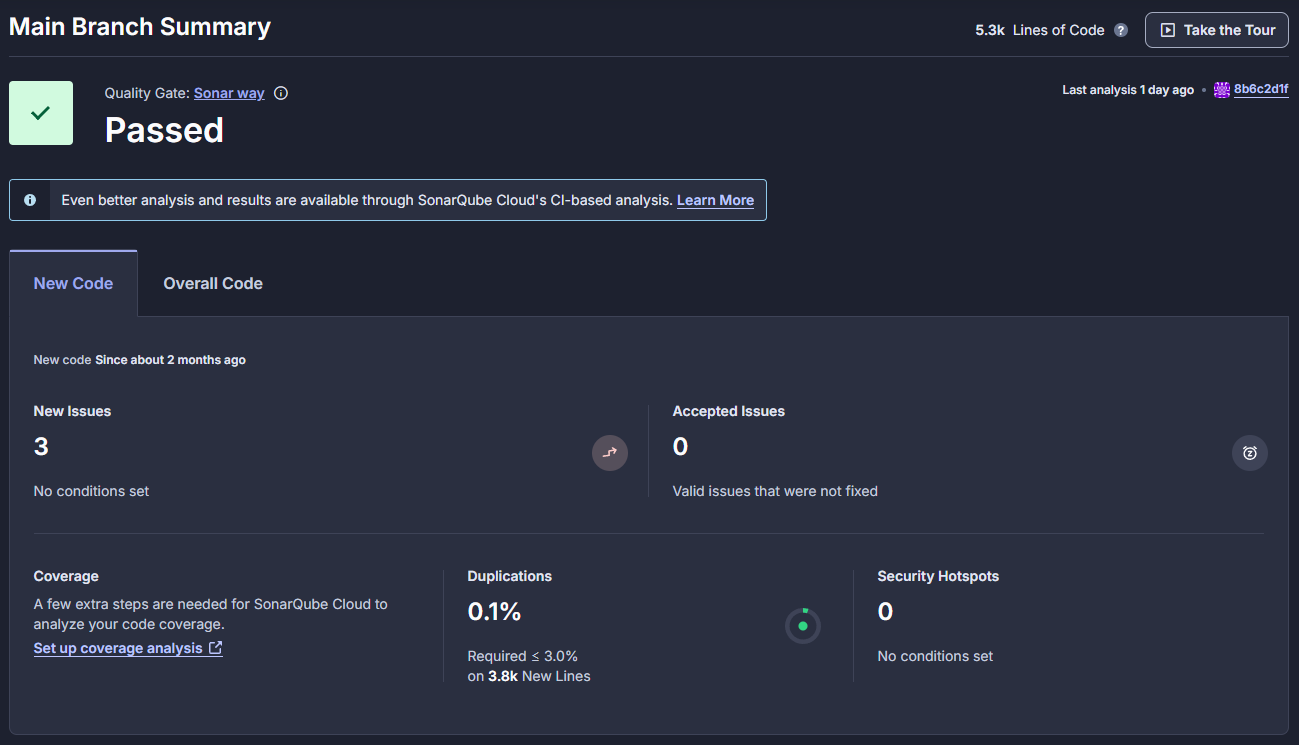
\includegraphics[width=\textwidth]{assets/code/sonarqube.png}
    }
    \caption{Schermata di Sonarqube Cloud}
    \label{fig:Sonarqube Cloud}
\end{figure}